\begin{center}
    \Large{\textbf{Практична частина}}
\end{center}

\vspace{1mm}

У результаті проведених експериментів 
були отримані наступні дослідні дані:

\begin{table}[h]
    \centering
    \begin{tabular}{|c|c|c|c|}
        \hline
        \textbf{Фільтр} & \textbf{Кільце} & \textbf{$r_{світ}$($10^{-5}$м)} & \textbf{$r_{тем}$($10^{-5}$м)} \\

        \hline
        \multirow{5}{*}{червоний} & 1 & 1 & 1.07 \\
        \cline{2-4}
        & 2 & 1.15 & 1.25 \\
        \cline{2-4}
        & 3 & 1.35 & 1.4 \\
        \cline{2-4}
        & 4 & 1.5 & 1.55 \\
        \cline{2-4}
        & 5 & 1.6 & 1.65 \\
        \hline
        
        \hline
        \multirow{5}{*}{помаранчевий} & 1 & 1 & 1.1 \\
        \cline{2-4}
        & 2 & 1.2 & 1.29  \\
        \cline{2-4}
        & 3 & 1.35 & 1.41 \\
        \cline{2-4}
        & 4 & 1.46 & 1.5  \\
        \cline{2-4}
        & 5 & 1.56 & 1.6  \\ 
        \hline

        \hline
        \multirow{5}{*}{зелений} & 1 & 0.93 & 1.03 \\
        \cline{2-4}
        & 2 & 1.12 & 1.17 \\
        \cline{2-4}
        & 3 & 1.25 & 1.31 \\
        \cline{2-4}
        & 4 & 1.36 & 1.41 \\
        \cline{2-4}
        & 5 & 1.44 & 1.50 \\
        \hline

        \hline
        \multirow{5}{*}{синій} & 1 & 0.99 & 1.08 \\
        \cline{2-4}        
        & 2 & 1.18 & 1.22 \\
        \cline{2-4}
        & 3 & 1.32 & 1.36 \\
        \cline{2-4}
        & 4 & 1.41 & 1.46 \\
        \cline{2-4}
        & 5 & 1.47 & 1.50 \\
        \hline

    \end{tabular}
    \caption{Дослідні дані}
\end{table}

З формул \ref{eq:4} і \ref{eq:5} бачимо, що значення радіуса 
кривизни $R$ та товщини зазору в місці контакту $d_0$ можна знайти 
розв'язав задачу лінійної регресіі, а саме, якщо $r^2 = k m + b$, то

$$ R = \frac{k}{\lambda} $$
$$ d_0 = - \frac{b_{тем}}{2R} = - \frac{b_{світ}}{2R} - \frac{\lambda}{4} $$

Діаметр плями, що утворилася міє лінзою та скляною поверхней, з елементарних
геометричних міркувань(теорема Піфагора) можна образувати наступним чином:

$$ D = 2 \sqrt{R^2 - (R-d_0)^2} = 2 \sqrt{2R|d_0| - d_0^2} $$

Отже, обрахуємо $R$, як середнє значення результатів для світлих і темних 
кілець. Результати містяться у таблиці 3(усі величини у мкм) Графіки отриманих залежносетй наведені нижче(рис. 2, рис. 3).

\begin{table}[h]
    \centering
    \begin{tabular}{|c|c|c|c|c|c|c|c|c|c|c|c|c|}
        \hline
        \textbf{Фільтр} & \textbf{$R_{тем}$} & \textbf{$R_{світ}$} & \textbf{$R$} &
        \textbf{$d_{0_{тем}}$} & \textbf{$d_{0_{світ}}$} & \textbf{$d_0$} & \textbf{$D$} \\
        \hline

        червоний & 1414.73 & 1433.25 & 1423.99 & -0.67 & -0.68 & -0.68 & 87.71 \\
        \hline
        
        помаранчевий & 1252.25 & 1356.25 & 1304.25 & -0.95 & -0.81 & -0.88 & 95.65 \\
        \hline
        
        зелений & 1372.44 & 1379.4 & 1375.92 & -0.71 & -0.7 & -0.7 & 87.89 \\
        \hline

        синій & 1618.89 & 1703.51 & 1661.2 & -0.72 & -0.67 & -0.7 & 96.15 \\
        \hline

    \end{tabular}
    \caption{Результати обчислень}
\end{table}



\begin{figure}[h!]    
    \centering
    \includegraphics[width=0.7\textwidth]{assets/r_dark(m).pdf}
    \caption{Графіки залежностей квадрату радіуса темних кілець від номера}
\end{figure}
\begin{figure}[h!]
    \centering
    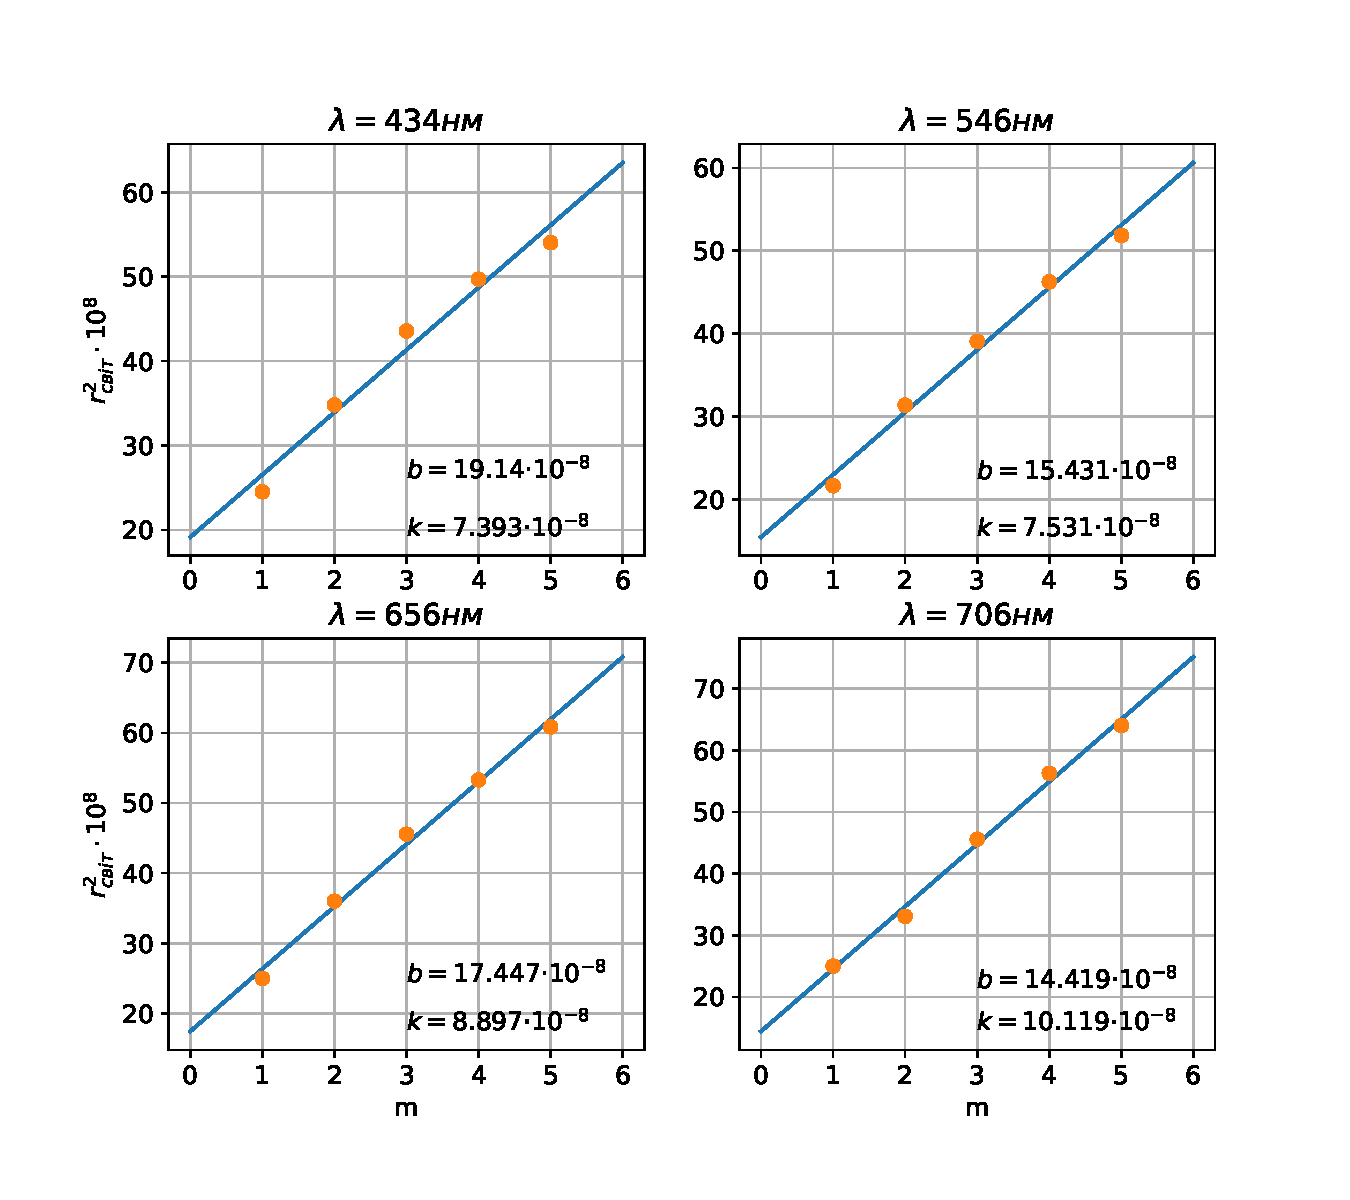
\includegraphics[width=0.7\textwidth]{assets/r_light(m).pdf}
    \caption{Графіки залежностей квадрату радіуса світлих кілець від номера}
\end{figure}

\pagebreak
Обчислимо абсолютні похибки за наступними формулами:

$$ \Delta R = $$
$$ \Delta D = $$

Покладаючи $\Delta r = 10^{-6}$, отримуємо наступні значення похибок.

\begin{table}[h!]
    \centering
    \begin{tabular}{|c|c|c|c|c|c|c|}
        \hline
        \textbf{Фільтр} & \textbf{$\Delta R$} & \textbf{$\Delta D$} &
        \textbf{$\varepsilon_R$} & \textbf{$\varepsilon_D$} \\
        \hline

        червоний &  & & &  \\
        \hline
        
        помаранчевий &  & &  &  \\
        \hline
        
        зелений & &  & &  \\
        \hline

        синій & &  & & \\
        \hline

    \end{tabular}
    \caption{Абсолютні та відносні похибки}
\end{table}